% make sure you have the VPN on, so that latex can load packages on the fly


\documentclass{article}

% graphics package
\usepackage{graphicx} 

% enhanced citation package 
\usepackage{natbib}
\bibpunct{(}{)}{;}{a}{}{,}  % to adjust punctuation in references


% adjust caption properties
\usepackage[margin=10pt, font=small, labelfont=bf]{caption} 

% hyperrefs on, with nicer colors
\usepackage{color}
\usepackage{xcolor}
\usepackage[]{hyperref}
\definecolor{darkblue}{rgb}{0,0,.5}
\hypersetup{colorlinks=true, breaklinks=true, linkcolor=darkblue, menucolor=darkblue, urlcolor=darkblue, citecolor=darkblue}

% enhanced tables
\usepackage{multicol}              
\usepackage{multirow}
\usepackage{booktabs}  


\author{Florian Hartig}
\title{My first \LaTeX document}

\begin{document}
\maketitle

\begin{abstract}
This document provides a first introduction into the typesetting system \LaTeX . After reading it, you will know everything there is to know about \LaTeX . 
\end{abstract}


\tableofcontents

\section{Introduction}


This is my \textbf{first} \emph{sentence}.

This is my \textit{second} sentence. 

This is my third sentence. You can also put some distance between lines.\\[3mm]
Test

\section{Doing equations}\label{sec: equations}

\subsection{Inline equations}
This is our first inline equation $\alpha = 3.5$. $\lambda = \sqrt{\alpha}$. 

\subsection{Numbered equations}

Test test

\begin{equation}
m = \left( \frac{a \cdot b}{c} \right) 
\end{equation}
%
where a = 5

\begin{equation}\label{eq: definition of lambda}
\lambda = \int_{m_0}^\infty f(\Theta) d \Theta
\end{equation}


\section{Labels and referencing}

In LaTeX, everything can be labeled, and after that it can be referenced. Consider for example section~\ref{sec: equations}, where eq.~\ref{eq: definition of lambda} are defined. You can also see this in fig.~\ref{fig: einstein}.

\section{Including figures}

\begin{figure}
\centering
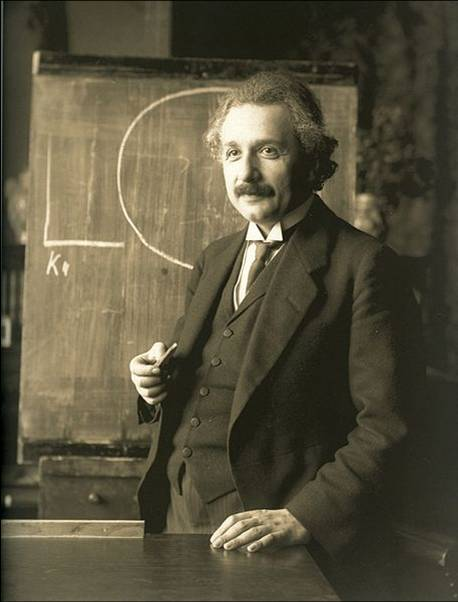
\includegraphics[width=6cm]{einstein} % without file extension
\caption{This shows Einstein in his study}\label{fig: einstein}
\end{figure}  

\begin{figure}
\centering
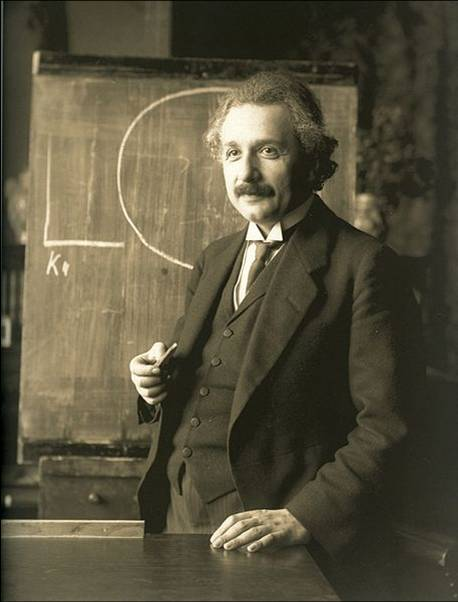
\includegraphics[width=3cm]{einstein}
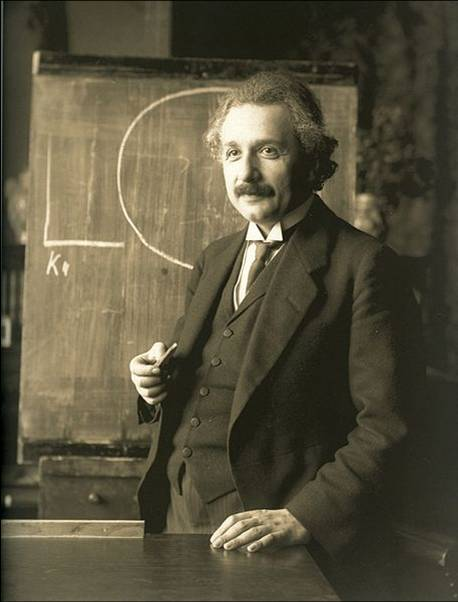
\includegraphics[width=3cm]{einstein}
\caption{This shows Einstein in his study}\label{fig: einstein2}
\end{figure}  



\begin{figure}
\centering
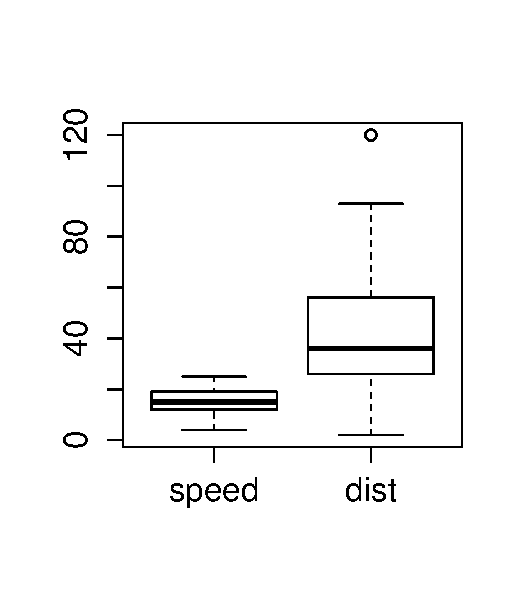
\includegraphics[width=6cm]{boxplot} % without file extension
\caption{This shows a boxplot}\label{fig: boxplot}
\end{figure} 

\section{Tables}

\subsection{Simple table}
\begin{tabular}{|c|c|}
\hline 
1 & 1 \\ 
\hline 
2 & 1 \\ 
\hline 
\end{tabular} 



\subsection{Proper table}



\begin{table*}\label{Table: Fit types}
  \centering
  \begin{tabular}{l@{\hspace{0.2cm}}l@{\hspace{0.2cm}}l} \toprule
  \textsc{Case} & \textsc{Explanation} & \textsc{Dimensions} \\ \midrule \addlinespace[0.2cm] 
  \multicolumn{3}{l}{Parameterization to virtual data, 3 PFTs:}  \\
  $V1$ & Data: SDD, GRO, reduced parameters &  $12,96$ \\ 
  $V2$ & Data: SDD, GRO, full parameters &  $26,96$  \\ 
  $V3$ & Data: SDD, reduced parameters &  $12,48$ \\ 
  $V4$ & Data: total SDD, reduced parameters &  $12,16$ \\ 
  $V5$ & Data: BM, reduced parameters &  $12,3$ \\  [0.2cm] 

  \multicolumn{3}{l}{Parameterization to Ecuadorian field data, 7 PFTs:} \\
  $E1$ & Data: SSD  &  $18,112$ \\ \bottomrule \\
\end{tabular}
\caption{Table caption}
\end{table*}


\section{References}

Referenced are extremely important \citep[see also][for more references]{Gintis-Costlysignalingand-2001,Archetti-Economicgametheory-2011}. However \citet{Cooper-CommunicationInCoordination-1992} note that this is not the case. 


% this is the style file. If you need to change something, google if the file you need is already there. If not (very uncommon) google makebst.
\bibliographystyle{chicago} 

% this is the bibtex libary file.
\bibliography{yourbibtexfile}

% Note: all files can be anywhere, just give the full path.


\end{document}
